\documentclass[../../main.tex]{subfiles}
\begin{document}

\begin{flushright}
  \footnotesize\textit{【自動文字起こし・要確認】}
\end{flushright}

% Source: handwritten.pdf 第6問．
{\bf [解答]}
地球の半径を1として良い．経路$R_1$は，半径$\cos\dfrac{\pi}{3}=\dfrac{1}{2}$の円周のうち
中心角$\dfrac{\pi}{3}$の扇形の弧長で，
\begin{align}R_1=\theta r=\dfrac{1}{2}\cdot\dfrac{1}{3}\pi=\dfrac{1}{6}\pi.\label{eq:1}
\end{align}
\begin{figure}[H]
  \centering
  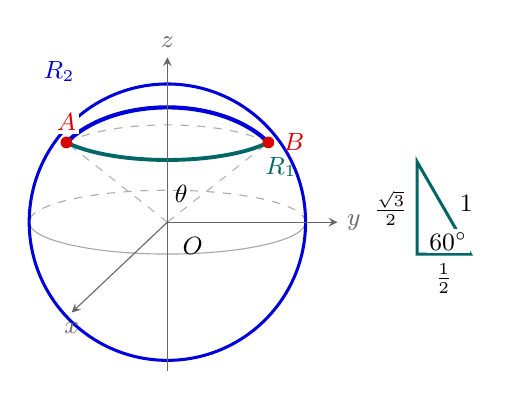
\begin{tikzpicture}[x=1.35cm,y=1.35cm,>=stealth,
    every node/.style={font=\small}]
    \coordinate (O) at (0,0);
    \coordinate (A) at (-.95,.75);
    \coordinate (B) at (.95,.75);
    \draw[gray!65,dashed] (1.3,0)
    arc[start angle=0,end angle=180,x radius=1.3,y radius=.3];
    \draw[gray!70] (-1.3,0)
    arc[start angle=180,end angle=360,x radius=1.3,y radius=.3];
    \draw[blue!85!black,line width=1.1pt] (O) circle (1.3);
    \draw[gray!65,dashed] (A) .. controls (-.5,.97) and (.5,.97) .. (B);
    \draw[gray!60,dashed] (O)--(A) (O)--(B);
    \draw[teal!80!black,line width=1.4pt]
    (A) .. controls (-.5,.53) and (.5,.53) .. (B);
    \draw[blue!85!black,line width=1.5pt]
    (A) .. controls (-.5,1.19) and (.5,1.19) .. (B);
    \draw[->,gray!80!black] (0,-1.4)--(0,1.55) node[above] {$z$};
    \draw[->,gray!80!black] (O)--(1.6,0) node[right] {$y$};
    \draw[->,gray!80!black] (O)--(-.9,-.85) node[below] {$x$};
    \node[circle, fill=red!85!black, inner sep=1.5pt] at (A) {}; \node[red!85!black, above=3pt, fill=white, inner sep=1pt] at (A) {$A$};
    \node[circle, fill=red!85!black, inner sep=1.5pt] at (B) {}; \node[red!85!black, right=2pt] at (B) {$B$};
    \node[below right=2pt] at (O) {$O$};
    \node[blue!85!black,above left=2pt] at (-.73,1.18) {$R_2$};
    \node[teal!80!black,right] at (.83,.52) {$R_1$};
    \node at (.13,.27) {$\theta$};
    \begin{scope}[shift={(2.35,-.3)}]
      \draw[teal!80!black,line width=1.1pt]
      (0,0)--(.5,0)--(0,.866)--cycle;
      \node[below] at (.25,0) {$\frac{1}{2}$};
      \node[left] at (0,.43) {$\frac{\sqrt{3}}{2}$};
      \node[right] at (.31,.48) {$1$};
      \node[above left,fill=white,inner sep=1pt] at (.5,0) {$60^\circ$};
    \end{scope}
  \end{tikzpicture}
  \caption{同一緯度の経路$R_1$と大円上の経路$R_2$の模式図}
\end{figure}
一方，$R_2$について，地球の中心を$O$として右のような座標をとれば
\begin{align}
  \overrightarrow{OA}=\dfrac{1}{2}
  \begin{pmatrix}1\\0\\\sqrt{3}
  \end{pmatrix},\qquad
  \overrightarrow{OB}=
  \begin{pmatrix}\dfrac{1}{4}\\\dfrac{\sqrt{3}}{4}\\\dfrac{\sqrt{3}}{2}
  \end{pmatrix}.
\end{align}
だから，$\angle AOB=\theta$として
\begin{align}
  \cos\theta=\dfrac{\overrightarrow{OA}\cdot\overrightarrow{OB}}{|\overrightarrow{OA}|\,|\overrightarrow{OB}|}
  =\dfrac{1}{2}
  \begin{pmatrix}1\\0\\\sqrt{3}
  \end{pmatrix}\cdot
  \dfrac{1}{4}
  \begin{pmatrix}1\\\sqrt{3}\\2\sqrt{3}
  \end{pmatrix}
  =\dfrac{7}{8}=0.875.
\end{align}
三角関数表から，
\begin{align}28.5^\circ<\theta<29.0^\circ.\label{eq:2}
\end{align}
\begin{align}R_2=\theta r=\theta.\label{eq:3}
\end{align}
したがって，\cref{eq:1,eq:3}より
\begin{align}\dfrac{R_2}{R_1}<\dfrac{29}{30}=0.96\cdots<0.97,\qquad R_2<0.97R_1
\end{align}
が示された．

\end{document}
